\documentclass[a4paper,twoside]{article}

\usepackage{epsfig}
\usepackage{subfigure}
\usepackage{calc}
\usepackage{amssymb}
\usepackage{amstext}
\usepackage{amsmath}
\usepackage{amsthm}
\usepackage{multicol}
\usepackage{pslatex}
\usepackage{apalike}
\usepackage{flushend}
\graphicspath{{figures/}}

\usepackage{SCITEPRESS}     % Please add other packages that you may need BEFORE the SCITEPRESS.sty package.

\newcommand{\anonymise}[1]{[Anonymised for review]}
\subfigtopskip=0pt
\subfigcapskip=0pt
\subfigbottomskip=0pt

\begin{document}

\title{Discover Insights from Cloud-based Applications based on Usage~Analytics}

\author{\authorname{\anonymise{Duc-Tien Dang-Nguyen, Manoj Kesavulu, and Markus Helfert}}
\affiliation{\anonymise{Lero –-- Irish Software Research Organization}}
\affiliation{\anonymise{School of Computing, Dublin City University, Dublin, Ireland}}
\email{\anonymise{\{duc-tien.dang-nguyen, markus.helfert\}@dcu.ie; manoj.kesavulu@lero.ie}}
}

\keywords{Usage Analytics, Cloud-based Applications, User Satisfaction, Resource Provision}

\abstract{This reports summarises state-of-the-art approaches for usage analytics of cloud-based application from usage data and point out the potential applications of this novel research direction.}

\onecolumn \maketitle \normalsize \vfill

\section{Introduction}\label{sec:Introduction}
%
%1 - Challenges in understanding performance on cloud environment.
Majority of the applications nowadays are moving to cloud-based environment, with the market size grows to $\$246.8B$ in 2017, according to Forbes\footnote{https://www.forbes.com/sites/louiscolumbus/2017/04/29/roundup-of-cloud-computing-forecasts-2017}. Users are using cloud-based services seamlessly, without recognising that they are not a desktop-based application. It, however, brings more challenges to people behind the systems to understand how the applications work and how their customer satisfy with the provided services. To have an example, let us recall the scenario of the cloud-based picture. Cloud providers deliver the same service to different customers, which share physical and/or virtual resources transparently. A cloud-based application lets customers share the same hardware resources, by offering them one shared application and database instance, while allowing them to configure the application to fit their needs as if it runs on a dedicated environment []. End-users or consumers interact with the cloud applications through various interfaces (those being web browsers, mobile applications, and command-line interfaces). Cloud services allows different users to share computing and virtual resources transparently, meanwhile guaranteeing substantial cost savings []. The Infrastructure as a Service (IaaS) model offers computer - physical or virtual machines - and other resources, such as raw block storage, file or object storage, virtual local area networks (VLANs), IP addresses, and firewalls. In the Software as a Service (SaaS) model, users can access applications and data. The more resources are managed by cloud providers, the more resources are shared by multiple different users. Extraction of usage data of the features provided by the cloud applications could help developers and architects to make an informed decision for the development/improvement of functionalities of the system according to end-user usage patterns []. 

%2 - Why do we need analytical solutions
Analytical solutions refer to the use of various analysis techniques (data mining, machine learning, reasoning, and etc.) to extract useful knowledge and insights from large data set. For example, enterprises can use analysis techniques to understand customers and predict which customers are least likely to quit, or most likely to respond to a particular offer based on their profiles, memberships they subscribe to, and their generated content (comments, clicks, etc.). Developers can understand if some functions do not work properly via the usage data generated by the users. Moreover, the resulting predictions can be used to generate lists of target customers or cases of interest, as input for strategic planning, or can be integrated into the context of other enterprise applications. Such analytical solutions are considered as increasingly important tools for modern enterprise to get an informational advantage, and have evolved from a matter of choice to a necessity in some crowded and competitive business landscapes. Applying analytical solutions, thus, is a key to discover insights from the applications. Traditionally, in order to understand how customers using a service, enterprises have to make a huge data collection via surveying and feedback from testers. With analytical solutions, such insights can be discovered via advance machine learning and data mining techniques from the usage data. 

Usage analytics aims to obtain insightful and actionable information for data-driven tasks, around applications and services. Insightful information is information that conveys meaningful and useful understanding or knowledge towards performing the target service or user satisfaction to that service \cite{Zhang2011}. Typically insightful information is not easily attainable by directly investigating the raw data without aid of analytical solutions. Actionable information is information upon which software practitioners can come up with concrete solutions (better than existing solutions if any) towards completing the target task. Developing a usage analytics project typically goes through iterations of the life cycle of four phases: task definition, data preparation, analytic-technology development, and deployment and feedback gathering. Task definition is to define the target task to be assisted by software analytics. Data preparation is to collect data to be analyzed. Analytic-technology development is to develop problem formulation, algorithms, and systems to explore, understand, and get insights from the data. Deployment and feedback gathering involves two typical scenarios. One is that, as researchers, we have obtained some insightful information from the data and we would like to ask domain experts to review and verify. The other is that we ask domain experts to use the analytic tools that we have developed to obtain insights by themselves. Most of the times it is the second scenario that we want to enable. Among various analytic technologies,machine learning is a well recognized technology for learning hidden patterns or predictive models from data. It plays an important role in software analytics. 

In this paper, we argue that when applying analytic technologies in practice of software analytics, one should:

- incorporate a broad spectrum of domain knowledge and expertise, e.g., management, machine learning, large-scale data processing and computing, and information visualization;
- investigate how practitioners take actions on the produced insightful and actionable information, and provide effective support for such information-based action taking.

To summarise, by using usage analytics, we are aiming at proposing powerful tools to address these challenges: 
%3 - What we can do with usage data analytics?
\begin{enumerate}
\item Resource provision
\item Problem diagnosis
\item User satisfaction
\item User behavior
\end{enumerate}

In this study, we summarise the big picture of how analytical solutions can be applied in cloud-based environments and answer some basis questions: 
\begin{itemize}
	\item ``What are the usage data?"
	\item ``What kind of insights can we get from the extracted data?"
	\item ``What kind of analytical techniques should be applied?"
\end{itemize}

\section{Problems, Challenges and Requirements}

\subsection{What are the usage data?}

System logs contain a wealth of information to help manage systems. Most systems print out  logs during their executions to record system runtime actions and states that can directly reflect system runtime behaviours. System developers and architects usually use these logs to track a system to detect and diagnose system anomalies. However, there are challenges in analyzing system logs in order to understand a system’s behaviors. 
% The program logic of a system usually has a lot of branches, and thus the system’s behaviors may be quite different under different input data or environmental conditions. Knowing the execution behavior under different inputs or configurations can greatly help system operators to understand system behaviors. However, there may be a large number of different combinations of inputs or parameters under different system behaviors. Such complexity poses difficulties for analyzing contextual information related to the state of interest. 
The user-level usage data in the context of this paper is the usage data generated as a result of user interaction with a cloud-based application. Some examples of usage data are  application logs, server logs, VM logs, Web cookies (from web browser), and so on. Such data in the cloud is spread across various interfaces such as Web browser, mobile apps and command line interfaces on the front-end and server and database on the back-end.  
% Generally, each log message consists of two different types of content: a constant string and parameter values. For example, for the first log-printing statement in Table 1, the constant string is “JVM with ID: given task:”, and the printed parameters are JvmId and TaskId. The log messages printed by the same log-print statement contain the same constant string, and are considered to be of the same type, represented by the constant string. 

As summary, there are mainly three sources of usage data can be extracted from the back-end of the cloud system: the system logs from the cloud services, the application logs, and the logs from the VMs. Fig.~\ref{fig:schema} shows a summary of the three main sources of usage data and the answers for the above questions.


\begin{figure*}[t!]
	\centering
	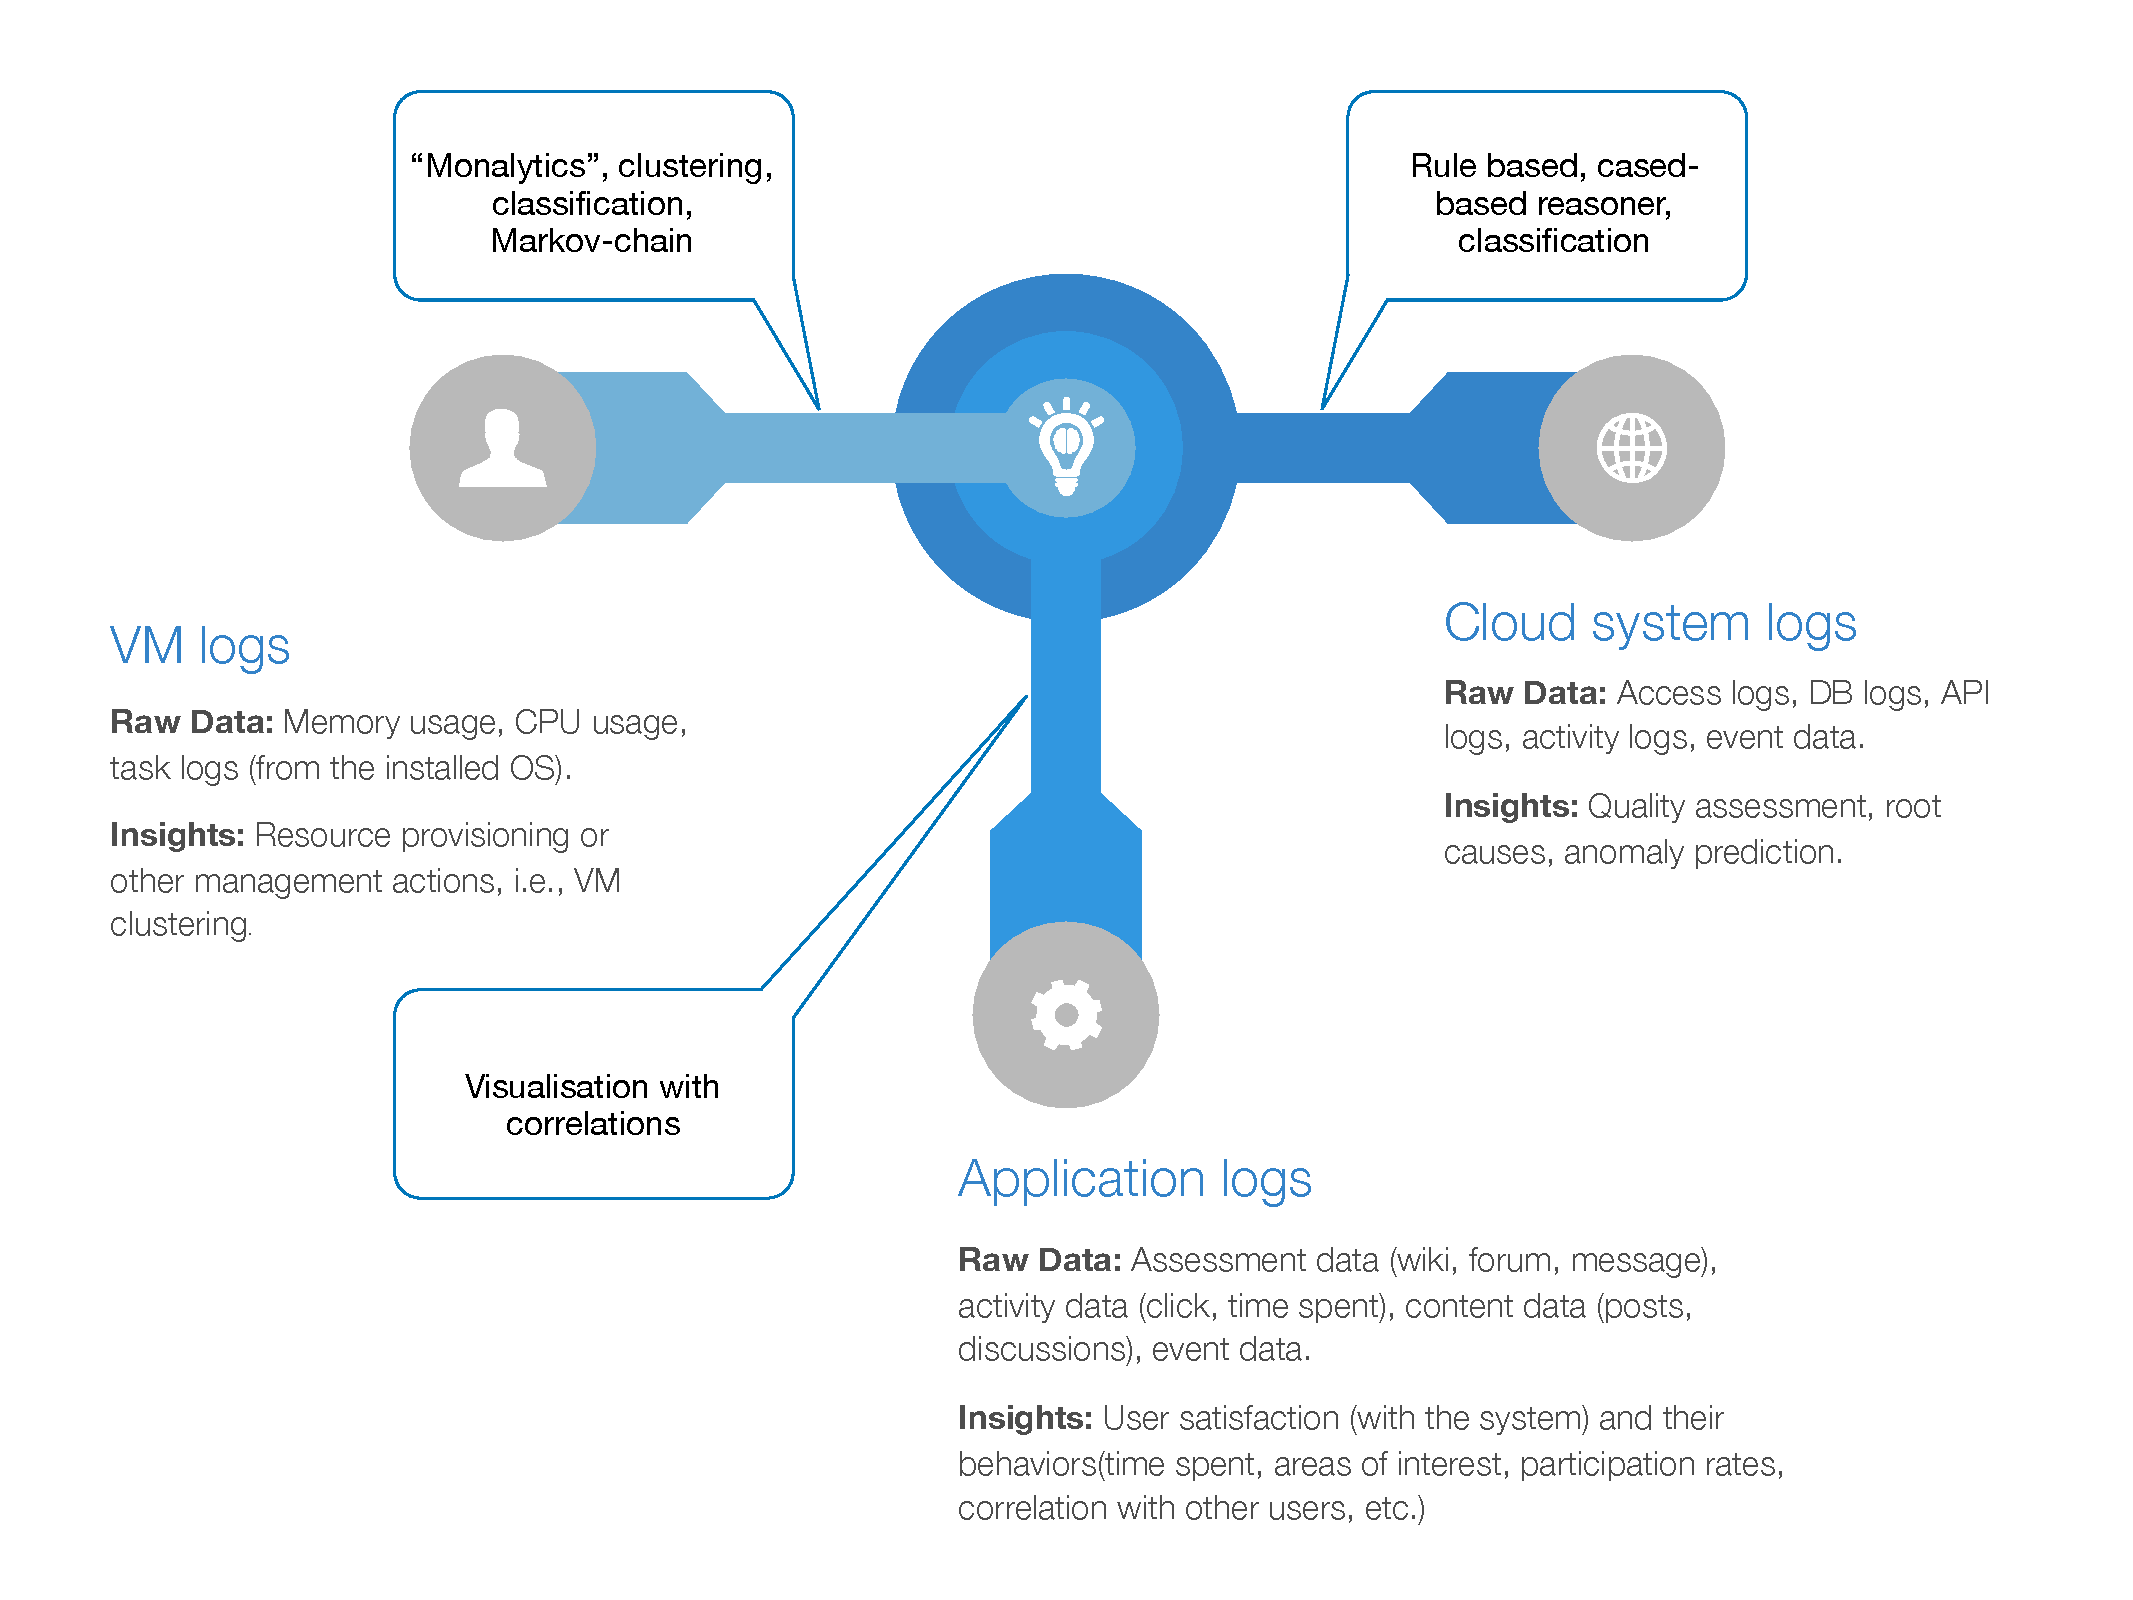
\includegraphics[width=\linewidth]{summary}
	\caption{Three main sources of usage data in cloud-based environment.}
	\label{fig:schema}
\end{figure*}

\subsection{Challenges in Extracting Information from Usage Data}

There are challenges in analyzing system logs in order to understand an end-user’s behaviors. The program logic of a system usually has a lot of branches, and thus the system’s behaviors may be quite different under different input data or environmental conditions. Knowing the execution behavior under different inputs or configurations can greatly help system operators to understand system behaviors. However, there may be a large number of different combinations of inputs or parameters under different system behaviors. Such complexity poses difficulties for analyzing contextual information related to the state of interest. Considering the multi-tenant architecture of the cloud, different applications share the same physical and virtual resources. This raises another challenge as in how to separate and extract the logs that represent each application from the instance (VM) co-hosting the applications. 
%
Since one of the ways to access the cloud-based applications by the end-user is through a web-browser, web-mining techniques can be employed to obtain interaction insights. \cite{Bucklin2009} provide an overview of \emph{Clickstream} data which is defined as the electronic record of a user's activity on the internet, this represents the data trace the path an end-user takes while accessing the cloud application. 

[] propose a new approach for the contextual analysis of program logs to better understand a system’s behaviors. In particular, they used execution patterns to represent the execution structures reflected by program logs, and propose an algorithm to mine execution patterns from the program logs. The mined execution patterns correspond to different execution paths of the system. Based on the execution patterns, their approach further learns the essential contextual factors (e.g., occurrences of specific program logs with specific parameter values) that cause a specific branch or path to be executed by the system. 
% * <manojpratnas@gmail.com> 2017-11-16T12:04:53.536Z:
% 
% Have to find the reference?
% 
% ^.
%
The mining and learning results can help system operators understand the execution logic and behaviors of a software system for their various maintenance tasks such as system problem diagnosis. This paper makes the following research contributions: We conduct Formal Concept Analysis (FCA) [4] to analyze log messages, and construct a concept lattice graph. The learned graph is used to mine execution patterns and to model relationships among different execution patterns. Such relationships represent branch structures in the program execution logic.

A huge wealth of various data exists in the software development process, and hidden in the data is information about the quality of software and services as well as the dynamics of software development. With various analytic technologies (e.g., data mining, machine learning, and information visualization), software analytics is to enable software practitioners to perform data exploration and analysis in order to obtain insightful and actionable information for data-driven tasks around applications and services.

\subsection{Challenges in Building Usage Analytics Framework}

Despite the advantages provided by analytical solutions, the solution implementation is usually very costly, which hinders enterprises, especially the SMBs (Small and Medium Business), to start such projects. Typically, an enterprise is required to first build a large storage system to store huge volumes of data collected from various data sources and channels; after that, the enterprise should buy expensive analytics software, and a large number of server machines, because the analytical programs often need mining huge amounts of data or executing complex learning algorithms. Moreover, the computational resource demand pattern of analytical solutions may be uneven with spikes (e.g., predicting product sale when a financial quarter is over or some unusual events happen), which means the enterprise has to pay a lot to maintain the complex software and hardware only for occasional usages. As a result, the systematical adoption of analytical solution is currently limited to only a small number of large enterprises. On the other hand, the analytical solution vendors also find it is difficult to deliver cost-effective solutions. Because analytical solutions require continuous model validation, tuning, and update according to the changing business context, it is hard for the solution vendors to control the travel expenditure in sending analysts to conduct incremental services in the customer site. In a word, a cost-effective delivery model becomes an important issue to accelerate the prevalence of analytical solutions. 

Currently, SaaS delivery model is well-studied to enable business clients consume applications at a low cost based on their usage [1], and cloud computing is considered as a promising technology to provide on demand storage and computational resources flexibly [2]. Accordingly, there are several relevant research efforts which have focused on leveraging these technologies to facilitate analytical solution delivery [3][4]. However, most of the projects are ad-hoc, that is, each of them is specific to a certain analytical application domain, and there is still lack of a comprehensive study to identify the differences between existing analytical solution delivery and analytics-as-a-service delivery, as well as a technical framework to handle the technical challenges introduced by the new delivery model.

\subsection{Analytics Requirements}
General requirements for an Analytics Engine (AE) are detailed below. 

A1. Data Source: AE must be able to fetch monitoring data recorded in the database. Further, it must be able to query the Cloud middlewares (e.g., that of OpenStack and OpenShift) and application APIs to know the current status of the services. 

A2. Proactive: AE must support the proactive management of resources. Proactive management needs short term and medium term predictions for the evolution of most relevant metrics. 

A3. Alerts: Certain QoS metrics need to be processed in real time and alerts should be triggered when these QoS metrics are violated or approach certain threshold values. 

A4. Event Correlation: Detecting the root cause of QoS faults and taking effective counter measures requires monitoring information spanning multiple tiers of the virtualized platforms. Quick in-comprehensive analysis of monitoring data of individual tiers does not reveal the root cause(s) of the problem precisely enough. Therefore, Analytics need to exhaustively aggregate runtime data from different sources and consolidate information at a high level of abstraction. 

A5: Identification of Influential Metrics: Identification of the metrics which strongly influence the QoS helps in decreasing the monitoring footprint and analysis complexity.

M1. Scalability: The MF should be scalable i.e. it can cope with a large number of monitoring data collectors. This requirement is very important in Cloud Computing scenarios due to a large number of parameters to be monitored for potentially large amount of services and elements of Cloud tiers that may grow elastically. 

M2. Heterogeneous data: The MF should consider a heterogeneous group of metrics. The MF must al- low the collection of service level runtime monitoring data, virtual IT-infrastructure monitoring data (e.g., VM level runtime monitoring), and fine-grained physical IT-infrastructure monitoring data (e.g., network links, computing and storage resources). 

M3. Polling Interval: The data collection mechanism must allow the dynamic customization of the polling interval. Dynamic nature of virtual platforms demands gathering of data in a sufficiently frequent manner, meaning that nodes should be monitored continuously. Naturally, smaller polling intervals introduce significant processing overhead inside nodes themselves. However, long polling intervals do not provide a clear picture of the monitored components. Therefore, an optimal trade-off between polling inter- val and processing overhead is required. 

M4. Relationship: In the above mentioned scenario, clusters of VMs and Physical Machines (PM) serve many kinds of applications, so there is a hierarchical relationship between applications, VMs and PMs.
There is also a possibility of migration of VMs and applications from one node to another, so relation- ships can be changed dynamically. Themetric’s value must be tagged to show that they belong to a particular instance (e.g., application), and what is their relation to other instances (e.g., VM and PM). 

M5. Data Repository: The MF requires a data repository where raw monitoring data needs to be stored after collection. The original data set must be stored without down-sampling for auditing purposes. The stored, raw monitoring data can be retrieved by consumers to perform QoS fault diagnosis, SLA validation, plot rendering, and as an input for fine grained resource management. The database must be distributed in order to avoid single point of failure. Moreover, it must be scalable, and allow to store thousands of metrics and potentially billions of data points. 

M6. Non-Intrusive: The MF must be able to retrieve data non-intrusively from a variety of sources (for VM via libvirt API, for a host via cgroups, for the network via SNMP, for Java applications via JMX, etc.). Collection mechanism should easily be extensible by adding more plugins. 

M7. Interface: The MF should provide a REST interface that allows access to the current monitoring data in a uniform and easy way, by abstracting the complexity of underlying monitoring systems. A standard unified interface for common management and monitoring tasks can make different virtualization technologies and Cloud providers interoperable. A REST interface is a good choice due to ease of implementation, low overhead and good scalability due to its session-less architecture.

\subsection{Evaluations and Validations}
Evaluation itself is a challenge in usage analytics. For example, if an analytical solution provides some information about the user satisfaction, it is nontrivial to evaluate if that information really show the real ``picture" of the satisfaction from the users. Traditionally, we need to run some surveys to evaluate results from the analytical solutions. Beside of that, in this study, we also propose a novel way for the evaluation by using another usage information, gathering from the snapshots of the users' device, for example screen-shots of the computer. By collecting these information (in the testing phase), we can provide users with the ability to recall and re-access their previous computer usage and the content they engage with. 

\section{The Proposed Solutions}
In this section, we describe the proposed analytics methods that aim to provide useful tools to solve the four major problems mentioned in the introduction: resource provision, problems diagnosis, understanding user satisfaction and user behaviours.

\subsection{Resource Provision}
Let us start with the left-most branch from diagram in Figure~\ref{fig:schema}. A typical problem on cloud-based environment is the networking capacity management, for example the Virtual Machine (VM) selections. A common problem experienced in data centers and utility clouds is lack of knowledge about the mappings of the services being run by or offered to external users to the sets of virtual machines (VMs) that implement them~\cite{Wang2011}. In order to solve this problem,  propose a system integrating monitoring with analytics, termed Monalytics, which can capture, aggregate, and incrementally analyze data on- demand and in real-time, only where (i.e., in situ) and to the extents needed by intended management actions. This is done by collecting CPU utilizations of VMs on each host. A central node gathering the data runs the lightweight clustering algorithms described in [9]. Its output is a list of potential VM ensembles, i.e., VMs that probably communicate regularly. 


The new overlay gathers IP package statistics from the VMs and analyzes total network traffic by using Top-K flow analysis [26]. The analysis finds the k flows that most contribute to the traffic between any two VMs and their sizes. It eliminates any member of the ensemble with coincidental correlations in terms of CPU usage, and provides the flow data needed to better assess the cost-benefits derived from VM migration.

 
 
 The restrictions caused by VM capacity predictions have limited the performances of most current cloud-based network management solutions~\cite{Sun2016}. It means that it is hard to obtain the values of the inputs for most existing planning approaches, even though most optimized techniques highly rely on the networking states [7], [8]. 
 
 We aim to propose a feasible method that efficiently predicts VM states that can be used as the inputs of the existing networking capacity management techniques. The outcomes of this work are significant for current enterprises that implement cloud-based applications by providing a panoramic view of the networking capacity management in different application scenarios.
 
 



\subsection{Problem Diagnosis}
With the increasing scale and complexity of software
systems, it has become more and more difficult for system operators to understand the behaviors of software systems for tasks such as system problem diagnosis. For example, system operators need to understand system behaviors to figure out why a software system is in the current status. With such an understanding, they can choose the right operations to achieve the desired goal. System behaviors include a series of actions executed by the system and the corresponding changes in the system states. Although operators usually investigate a system starting from a specific state of interest, e.g., a hang state or failure state, contextual information for reaching that state is critical for identifying why the system runs in that state. Such contextual information includes how previous actions are executed by the system, what the historical system states are before running into the state of interest, what the input data is, etc.


Today more and more (monolithic) applications are decomposed into smaller components which are then executed as services on virtualized platforms connected via network communication and orchestrated to deliver the desired functionality. While the foundations for decomposing, executing and orchestrating were well settled over the past decade, allocating the needed resources for and steering the execution of components to deliver the required Quality of Service (QoS) is an active area of research. A critical aspect of steering complex service-based applications on virtualized platforms is effective, non-intrusive, low-footprint monitoring of key performance indicators at different provisioning tiers typically Infrastructure- as-a-Service, Platform-as-a-Service and Software-as- a-Service. These key performance indicators are assessed to verify that a Service Level Agreement (SLA) between a customer and a provider is met. Ideally, the assessment goes beyond simply detecting violations of the agreed terms, but tries to predict and preempt potential violations. The provider enacts counter-measures to prevent or resolve the violation if it does occur. Deriving effective counter-measures requires precise monitoring information spanning multiple tiers of the virtualized platform and analysis of monitoring data to identify the root cause(s) of performance problems.

Monitoring systems have been used over decades in different computing paradigms. Monitoring solutions for previous computing paradigms pose significant limitations for their widespread adoption in large scale, virtual platforms. The major obstacles with these monitoring techniques are, their high performance overhead, reliability, isolation, limited scalability, reliance on proprietary protocols and technologies.

Common performance diagnosis procedures depend on system administrator’s domain knowledge and associated performance best practices. This procedure is labor intensive, error prone, and not feasible for virtual platforms. The prior art on detecting and diagnosing faults in computing systems can be reviewed in (Appleby et al., 2001) (Molenkamp, 2002) (Agarwal et al., 2004) (Chen et al., 2002)(Barham et al., 2003). These methods do not consider virtualization technologies and are inappropriate for rapidly changing, large scale virtual platforms that by very nature require effective automated techniques for QoS fault diagnosis.

Our research motivations are to study the effectiveness and practicality of different techniques for performance problem diagnosis and SLA based re- source management of virtual platforms. 


\subsection{Understanding User Behavior}


\subsection{Understanding User Satisfaction}
There are two main categories of challenges to overcome in or-
der to achieve the stated objectives. The first category is rooted from the characteristics of the data being analyzed with analytic technologies. Data scale. Typical data in software analytics is of large scale,
e.g., due to the large scale of software being developed and the large size of software development teams. Some tasks require to analyze division-wide or even company-wide code bases, which are far be- yond the scope of a single code base (e.g., when conducting code- clone detection [2]). Some tasks require to analyze a large quantity of (likely noisy) data samples within or beyond a single code base (e.g., when conducting runtime-trace analysis [3]). Although lack- ing data samples may not be an issue in this context of machine learning, the large scale of data poses challenges for data process- ing and analysis, including learning-algorithm design and system building. Data complexity. Typical data in software analytics is of high
complexity, which is partly due to the high complexity of software being developed. For example, runtime traces fromdistributed sys- tems [3] need to be correlated, while traces frommultiple threads [7] need to be split. System logs [3] include unstructured textual in- formation. There could be high dependencies across traces and noises among traces. In addition, real-world usage data produced from in-field operations offers substantial opportunities for various tasks such as debugging (e.g., those assisted by the Microsoft Er- ror Reporting system [4]). In addition to high complexity, such data is typically distributed and often partial (e.g., collected with sampling-based techniques to reduce runtime overhead). All these characteristics pose challenges for analytic technologies such as machine learning. The second category is rooted from the characteristics of the
tasks being assisted by software analytics. Focus on ultimate tasks being assisted. Among tasks assisted
by software analytics, some tasks are intermediate tasks and some are ultimate tasks. Usually intermediate tasks produce information toward solving ultimate tasks. For example, code-clone detection is considered as an intermediate task, which produces information towards refactoring and defect detection that are ultimate tasks.

Such focus on ultimate tasks requires the mandatory inclusion of the phase of deployment and feedback gathering in the life cycle of a software analytic project. Unlike most previous research on code-clone detection, we should not stop at measuring the preci- sion and recall of detected clones; rather, we should push further to accomplish that the detected clones could effectively help address ultimate tasks such as refactoring and defect detection, and should measure such benefits in evaluations. Engagement of customers during the development process of a
software analytic project. It is well recognized that engaging cus- tomers is a challenging task especially in the context of software engineering tools. Customers may have resistance to proposed changes (due to analytic-tool adoption) on their existing way of carrying out a task. In addition, due to tight development sched- ule, they may not be able to invest time on gaining understanding of the best/worst scenarios for applying an analytic tool. However, developing a software analytic project typically needs the engage- ment of customers in iterations of the four phases in the project life cycle, e.g., to get better understanding on the tasks and domain knowledge. Among the phases, especially the phase of deployment and feedback gathering, it is crucial for the produced analytic tools to have good usability, e.g., providing effective visualization and manipulation of analysis results.




\section{Discussions}

M1. Scalability: The MF should be scalable i.e. it can cope with a large number of monitoring data collectors. This requirement is very important in Cloud Computing scenarios due to a large number of parameters to be monitored for potentially large amount of services and elements of Cloud tiers that may grow elastically. 

M2. Heterogeneous data: The MF should consider a heterogeneous group of metrics. The MF must al- low the collection of service level runtime monitoring data, virtual IT-infrastructure monitoring data (e.g., VM level runtime monitoring), and fine-grained physical IT-infrastructure monitoring data (e.g., network links, computing and storage resources). 

M3. Polling Interval: The data collection mechanism must allow the dynamic customization of the polling interval. Dynamic nature of virtual platforms demands gathering of data in a sufficiently frequent manner, meaning that nodes should be monitored continuously. Naturally, smaller polling intervals introduce significant processing overhead inside nodes themselves. However, long polling intervals do not provide a clear picture of the monitored components. Therefore, an optimal trade-off between polling inter- val and processing overhead is required. 

M4. Relationship: In the above mentioned scenario, clusters of VMs and Physical Machines (PM) serve many kinds of applications, so there is a hierarchical relationship between applications, VMs and PMs.
There is also a possibility of migration of VMs and applications from one node to another, so relation- ships can be changed dynamically. Themetric’s value must be tagged to show that they belong to a particular instance (e.g., application), and what is their relation to other instances (e.g., VM and PM). 

M5. Data Repository: The MF requires a data repository where raw monitoring data needs to be stored after collection. The original data set must be stored without down-sampling for auditing purposes. The stored, raw monitoring data can be retrieved by consumers to perform QoS fault diagnosis, SLA validation, plot rendering, and as an input for fine grained resource management. The database must be distributed in order to avoid single point of failure. Moreover, it must be scalable, and allow to store thousands of metrics and potentially billions of data points. 

M6. Non-Intrusive: The MF must be able to retrieve data non-intrusively from a variety of sources (for VM via libvirt API, for a host via cgroups, for the network via SNMP, for Java applications via JMX, etc.). Collection mechanism should easily be extensible by adding more plugins. 

M7. Interface: The MF should provide a REST interface that allows access to the current monitoring data in a uniform and easy way, by abstracting the complexity of underlying monitoring systems. A standard unified interface for common management and monitoring tasks can make different virtualization technologies and Cloud providers interoperable. A REST interface is a good choice due to ease of implementation, low overhead and good scalability due to its session-less architecture.

\section{Realising the Potential}
All these potential held by --- comes also with challenges and opportunities for researchers.
It is important that the multimedia community helps to address the challenges in this emerging and important field. 
We cannot easily apply our existing methods on this type of data and hope for access. Therefore we need specific
approaches addressing the specific challenges.
As a first way-point for researchers we are proposing different research topics and research questions.
\begin{enumerate}
	\item How can we identify and extract important information? Deciding what should be extracted from the data that is important for the users is a nontrivial task. Going beyond standard analysis like detecting visual objects or text will be important, forcing researchers to think creatively and go beyond simple analysis. Many research questions arises, such as, how to combine information from sensors with videos or images, or how to efficiently process the data. Also an important part here is to explore how context can be taken into account to improve the quality of the analysis.
	
	\item How can we present the results to the users? 
	Reporting the results to the users is one of the most important parts of the analysis of this data. Nevertheless, this is not trivial since the amount of data and information that can be extracted is huge. It will be important to research novel interfaces that allow users to browse efficiently. Apart from that user feedback loops and recommender systems that can help the user to decide which information is important to them. Finally, generating summaries and automatic reports will be another topic that is important for this data since there will be a need from the user side for such summaries with respect to, for example, weekly report from sensors such as Fitbit smartwatches.
	
	\item How can and which technologies are need to make it easy to share, annotate and archive data? 
	While services similar to YouTube or Flickr might be interesting for users, it also comes with a privacy problem. Users might want to upload and share there data but in a more controlled way. New ways of secure sharing but also tools for annotating, redaction, and archiving large amounts of data will be needed. With this also comes the need for re-finding certain events which bring new challenges for search engines.  
	
	\item How can information and data be processed efficiently? Systems that have to process a huge amount of data in a complex way have to be efficient to make them useful to the users. This comes with challenges for multimedia systems researchers in terms of how to parallelize and process data efficiently in a reasonable amount of time.
\end{enumerate}

The potential for personal life archives is enormous. We do acknowledge that there are  challenges to be overcome, such as privacy concerns, data storage, security of data, and the development of a new generation of search and organisation tools, but we believe that these will be overcome and that we are on the cusp of a positive turning point for society; the era of the quantified individual who knows more about the self than ever before, has more knowledge to improve the quality of their own life and can share life events and experiences in rich detail with friends and contacts.

\section{Conclusions}
In this paper we presented the challenges in getting insights from cloud based applications. We pointed out analytical solutions of how to overcome these challenges by exploiting the usage data. Some potential applications were also discussed.

\section*{\uppercase{Acknowledgements}}
\noindent This work was supported with the financial support of the \anonymise{Science Foundation Ireland grant 13/RC/2094} and co-funded under the \anonymise{European Regional Development Fund through the Southern \& Eastern Regional Operational Programme} to \anonymise{Lero - the Irish Software Research Centre (www.lero.ie)}.

%\vfill
\bibliographystyle{apalike}
{\small
\bibliography{refs}}

%
%\section*{\uppercase{Appendix}}

%\noindent If any, the appendix should appear directly after the
%references without numbering, and not on a new page. To do so please use the following command:
%\textit{$\backslash$section*\{APPENDIX\}}

%\vfill
\end{document}

